% !Mode:: "TeX:UTF-8"

\documentclass[12pt,openany,oneside]{book}

\input{setup/package} % 定义所需宏包

\begin{document}
% !Mode:: "TeX:UTF-8"
% Author: Unlucky
% Blog: http://unlucky.orgfree.com/blog

%%%%%%%%%% Fonts Definition and Basics %%%%%%%%%%%%%%%%%
\XeTeXlinebreaklocale "zh"
\XeTeXlinebreakskip = 0pt plus 1pt minus 0.1pt
\setCJKfamilyfont{song}{SimSun}             % 宋体
\newcommand{\song}{\CJKfamily{song}}
\setCJKfamilyfont{fs}{FangSong}             % 仿宋体
\newcommand{\fs}{\CJKfamily{fs}}
\setCJKfamilyfont{kai}{KaiTi}               % 楷体
\newcommand{\kai}{\CJKfamily{kai}}
\setCJKfamilyfont{hei}{SimHei}              % 黑体
\newcommand{\hei}{\CJKfamily{hei}}
\setCJKfamilyfont{li}{LiSu}                 % 隶书
\newcommand{\li}{\CJKfamily{li}}
\setCJKfamilyfont{tnroman}{Times New Roman} % Times New Roman
\newcommand{\tnroman}{\CJKfamily{tnroman}}

\newcommand{\yihao}{\fontsize{26pt}{26pt}\selectfont}       % 一号, 单倍行距
\newcommand{\xiaoyi}{\fontsize{24pt}{24pt}\selectfont}      % 小一, 单倍行距
\newcommand{\erhao}{\fontsize{22pt}{27.5pt}\selectfont}       % 二号, 1.25倍行距
\newcommand{\xiaoer}{\fontsize{18pt}{18pt}\selectfont}      % 小二, 单倍行距
\newcommand{\sanhao}{\fontsize{16pt}{16pt}\selectfont}      % 三号, 单倍行距
\newcommand{\xiaosan}{\fontsize{15pt}{22.5pt}\selectfont}     % 小三, 单倍行距
\newcommand{\sihao}{\fontsize{14pt}{14pt}\selectfont}       % 四号, 单倍行距
\newcommand{\xiaosi}{\fontsize{12pt}{18pt}\selectfont}      % 小四, 单倍行距
\newcommand{\wuhao}{\fontsize{10.5pt}{10.5pt}\selectfont}   % 五号, 单倍行距
\newcommand{\xiaowu}{\fontsize{9pt}{9pt}\selectfont}        % 小五, 单倍行距

\setCJKmainfont{SimSun}
\setCJKmonofont{SimSun}
\setmainfont{Times New Roman}

% \CJKcaption{gb_452}
% \CJKtilde  % 重新定义了波浪符~的意义
\newcommand\prechaptername{第}
\newcommand\postchaptername{章}

% \punctstyle{plain}
% 调整罗列环境的布局
\setitemize{leftmargin=3em,itemsep=0em,partopsep=0em,parsep=0em,topsep=-0em}
\setenumerate{leftmargin=3em,itemsep=0em,partopsep=0em,parsep=0em,topsep=0em}
% \setlength{\baselineskip}{20pt}
% \renewcommand{\baselinestretch}{1.38} % 设置行距

% 避免宏包 hyperref 和 arydshln 不兼容带来的目录链接失效的问题。
\def\temp{\relax}
\let\temp\addcontentsline
\gdef\addcontentsline{\phantomsection\temp}

% 自定义项目列表标签及格式 \begin{publist} 列表项 \end{publist}
\newcounter{pubctr} %自定义新计数器
\newenvironment{publist}{%%%%%定义新环境
  \begin{list}{[\arabic{pubctr}]} %%标签格式
    {
      \usecounter{pubctr}
      \setlength{\leftmargin}{2.5em}   % 左边界 \leftmargin =\itemindent + \labelwidth + \labelsep
      \setlength{\itemindent}{0em}     % 标号缩进量
      \setlength{\labelsep}{1em}       % 标号和列表项之间的距离,默认0.5em
      \setlength{\rightmargin}{0em}    % 右边界
      \setlength{\topsep}{0ex}         % 列表到上下文的垂直距离
      \setlength{\parsep}{0ex}         % 段落间距
      \setlength{\itemsep}{0ex}        % 标签间距
      \setlength{\listparindent}{0pt} % 段落缩进量
    }}
  {\end{list}}%%%%%

\makeatletter
\renewcommand\normalsize{
  \@setfontsize\normalsize{12pt}{12pt} % 小四对应12pt
  \setlength\abovedisplayskip{4pt}
  \setlength\abovedisplayshortskip{4pt}
  \setlength\belowdisplayskip{\abovedisplayskip}
  \setlength\belowdisplayshortskip{\abovedisplayshortskip}
  \let\@listi\@listI}
\def\defaultfont{\renewcommand{\baselinestretch}{1.38}\normalsize\selectfont}
% 设置行距和段落间垂直距离
\renewcommand{\CJKglue}{\hskip 0.96pt plus 0.08\baselineskip} %加大字间距,使每行33个字

\makeatother
%%%%%%%%%%%%% Contents %%%%%%%%%%%%%%%%%
% 主目录设置
\renewcommand{\contentsname}{目\qquad 录}
\setcounter{tocdepth}{1}
\titlecontents{chapter}[2em]{\vspace{.5\baselineskip}\xiaosan\song}%
{\prechaptername\CJKnumber{\thecontentslabel}\postchaptername\qquad}{} %
{\hspace{.5em}\titlerule*[10pt]{$\cdot$}\sihao\contentspage}
\titlecontents{section}[3em]{\vspace{.25\baselineskip}\sihao\song} %
{\thecontentslabel\quad}{} %
{\hspace{.5em}\titlerule*[10pt]{$\cdot$}\sihao\contentspage}
\titlecontents{subsection}[4em]{\vspace{.25\baselineskip}\xiaosi\song} %
{\thecontentslabel\quad}{} %
{\hspace{.5em}\titlerule*[10pt]{$\cdot$}\sihao\contentspage}

% 图目录设置
\renewcommand{\listfigurename}{图目录}
\newcommand{\loflabel}{图}
\renewcommand{\numberline}[1]{\loflabel~#1\hspace*{1em}}

% 表目录设置
\renewcommand{\listtablename}{表目录}
\newcommand{\lotlabel}{表}
\renewcommand{\numberline}[1]{\lotlabel~#1\hspace*{1em}}


%%%%%%%%%% Chapter and Section %%%%%%%%%%%%%%%%%
\setcounter{secnumdepth}{4}
\setlength{\parindent}{2em}
\renewcommand{\chaptername}{\prechaptername\CJKnumber{\thechapter}\postchaptername}
\titleformat{\chapter}{\centering\xiaosan\bfseries}{\chaptername}{2em}{}
\titlespacing{\chapter}{0pt}{0.3\baselineskip}{1\baselineskip}
\titleformat{\section}{\sihao\bfseries}{\thesection}{1em}{}
\titlespacing{\section}{0pt}{0.2\baselineskip}{0.5\baselineskip}
\titleformat{\subsection}{\sihao\bfseries}{\thesubsection}{1em}{}
\titlespacing{\subsection}{0pt}{0.1\baselineskip}{0.3\baselineskip}
\titleformat{\subsubsection}{\sihao\bfseries}{\thesubsubsection}{1em}{}
\titlespacing{\subsubsection}{0pt}{0}{0}

%%%%%%%%%% Table, Figure and Equation %%%%%%%%%%%%%%%%%
\renewcommand{\tablename}{表} % 插表题头
\renewcommand{\figurename}{图} % 插图题头
\renewcommand{\thefigure}{\arabic{chapter}-\arabic{figure}} % 使图编号为 7-1 的格式 %\protect{~}
\renewcommand{\thesubfigure}{\alph{subfigure})}%使子图编号为 a)的格式
\renewcommand{\thesubtable}{(\alph{subtable})} %使子表编号为 a)的格式
\renewcommand{\thetable}{\arabic{chapter}-\arabic{table}}%使表编号为 7-1 的格式
\renewcommand{\theequation}{\arabic{chapter}-\arabic{equation}}%使公式编号为 7-1 的格式

%% 定制浮动图形和表格标题样式
\makeatletter
\long\def\@makecaption#1#2{%
  \vskip\abovecaptionskip
  \sbox\@tempboxa{\centering\wuhao\song{#1\qquad #2} }%
  \ifdim \wd\@tempboxa >\hsize
  \centering\wuhao\song{#1\qquad #2} \par
  \else
  \global \@minipagefalse
  \hb@xt@\hsize{\hfil\box\@tempboxa\hfil}%
  \fi
  \vskip\belowcaptionskip}
\makeatother
\captiondelim{~~~~} %用来控制longtable表头分隔符

%%%%%%%%%% Theorem Environment %%%%%%%%%%%%%%%%%
\theoremstyle{plain}
\theorembodyfont{\song\rmfamily}
\theoremheaderfont{\hei\rmfamily}
\newtheorem{theorem}{定理~}[chapter]
\newtheorem{lemma}{引理~}[chapter]
\newtheorem{axiom}{公理~}[chapter]
\newtheorem{proposition}{命题~}[chapter]
\newtheorem{corollary}{推论~}[chapter]
\newtheorem{definition}{定义~}[chapter]
\newtheorem{conjecture}{猜想~}[chapter]
\newtheorem{example}{例~}[chapter]
\newtheorem{remark}{注~}[chapter]
\newtheorem{algorithm}{算法~}[chapter]
\newenvironment{proof}{\noindent{\hei 证明:}}{\hfill $ \square $ \vskip 4mm}
\theoremsymbol{$\square$}

%%%%%%%%%% Page: number, header and footer  %%%%%%%%%%%%%%%%%

% \frontmatter 或 \pagenumbering{roman}
% \mainmatter 或 \pagenumbering{arabic}
\makeatletter
\renewcommand\frontmatter{\clearpage
  \@mainmatterfalse
  \pagenumbering{Roman}} % 正文前罗马字体编号
\makeatother


%%%%%%%%%% References %%%%%%%%%%%%%%%%%
\renewcommand{\bibname}{参考文献}
% 重定义参考文献样式,来自thu
\makeatletter
\renewenvironment{thebibliography}[1]{%
  \titleformat{\chapter}{\raggedright\sihao\hei}{\chaptername}{2em}{}
  \chapter*{\bibname}%
  \wuhao
  \list{\@biblabel{\@arabic\c@enumiv}}%
  {\renewcommand{\makelabel}[1]{##1\hfill}
    \settowidth\labelwidth{0.5cm}
    \setlength{\labelsep}{0pt}
    \setlength{\itemindent}{0pt}
    \setlength{\leftmargin}{\labelwidth+\labelsep}
    \addtolength{\itemsep}{-0.7em}
    \usecounter{enumiv}%
    \let\p@enumiv\@empty
    \renewcommand\theenumiv{\@arabic\c@enumiv}}%
  \sloppy\frenchspacing
  \clubpenalty4000%
  \@clubpenalty \clubpenalty
  \widowpenalty4000%
  \interlinepenalty4000%
  \sfcode`\.\@m}
{\def\@noitemerr
  {\@latex@warning{Empty `thebibliography' environment}}%
  \endlist\frenchspacing}
\makeatother

\addtolength{\bibsep}{-0.5em} % 缩小参考文献间的垂直间距
\setlength{\bibhang}{2em} %每个条目自第二行起缩进的距离

% 参考文献引用作为上标出现
% \newcommand{\citeup}[1]{\textsuperscript{\cite{#1}}}
\makeatletter
\def\@cite#1#2{\textsuperscript{[{#1\if@tempswa , #2\fi}]}}
\makeatother
%% 引用格式
\bibpunct{[}{]}{,}{s}{}{,}

%%%%%%%%%% Cover %%%%%%%%%%%%%%%%%
% 封面、摘要、版权、致谢格式定义
\makeatletter
\def\ctitle#1{\def\@ctitle{#1}}\def\@ctitle{}
\def\caffil#1{\def\@caffil{#1}}\def\@caffil{}
\def\csubject#1{\def\@csubject{#1}}\def\@csubject{}
\def\cauthor#1{\def\@cauthor{#1}}\def\@cauthor{}
\def\csupervisor#1{\def\@csupervisor{#1}}\def\@csupervisor{}
\def\cdate#1{\def\@cdate{#1}}\def\@cdate{}
\long\def\cabstract#1{\long\def\@cabstract{#1}}\long\def\@cabstract{}
\long\def\eabstract#1{\long\def\@eabstract{#1}}\long\def\@eabstract{}
\def\ckeywords#1{\def\@ckeywords{#1}}\def\@ckeywords{}
\def\ekeywords#1{\def\@ekeywords{#1}}\def\@ekeywords{}
\def\cheading#1{\def\@cheading{#1}}\def\@cheading{}

% 在book文件类别下,\leftmark自动存录各章之章名,\rightmark记录节标题
\pagestyle{fancy}
% 去掉章节标题中的数字 务必放到\pagestyle{fancy}之后才会起作用
%% 不要注销这一行,否则页眉会变成:“第1章1  绪论”样式
\renewcommand{\chaptermark}[1]{\markboth{\chaptername~\ #1}{}}
\fancyhf{}
% \fancyhead[C]{\song\wuhao \leftmark} % 页眉显示章节名称
\fancyhead[C]{\song\xiaowu \@cheading}
% \fancyhead[CO]{\song\wuhao \@cheading}
% \fancyhead[CE]{\song\wuhao \@cheading}
\fancyfoot[C]{\song\xiaowu ~\thepage~}

\fancypagestyle{plain}{% 设置开章页页眉页脚风格
  \fancyhf{}%
  % \fancyhead[C]{\song\wuhao \leftmark}
  \fancyhead[C]{\song\xiaowu \@cheading}
  \fancyfoot[C]{\song\xiaowu ~\thepage~ } %%首页页脚格式
  \renewcommand{\headrulewidth}{0.5pt}%
  \renewcommand{\footrulewidth}{0pt}%
}

% 定义封面
\def\makecover{
  % \cleardoublepage%
  \phantomsection
  \pdfbookmark[-1]{\@ctitle}{ctitle}

  \begin{titlepage}
  	\vspace*{-2.5mm}
    \begin{center}
      %校名
      \begin{figure}[h]
        \centering
        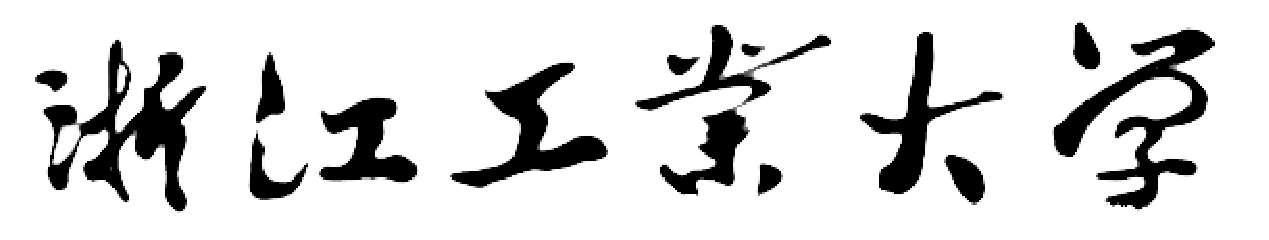
\includegraphics[width=9.84cm]{figures/zjut}
      \end{figure}
      \vspace*{9.66mm}
	  \song\yihao{本科毕业设计说明书(论文)}\\
	  \vspace*{10.0mm}
	  \song\xiaoer\bf{(2013届)}\\
      \vspace*{8.5mm}
      %校徽
      \begin{figure}[h]
        \centering
        
\includegraphics[width=2.73cm]{figures/zjutlogo}
      \end{figure}
      \vspace*{0.0mm}
      \renewcommand{\arraystretch}{1.0}
      \begin{tabular}{lc}
        \song\erhao{论文题目\quad} & \song\xiaoer{\@ctitle} \\ \cline{2-2}
      \end{tabular}\\
	  \vspace*{11.1mm}
      \setlength{\arrayrulewidth}{0.5pt}
      {\song\sihao
        \renewcommand{\arraystretch}{2.0}
        \begin{tabular}{lc}
          作者姓名\qquad &  \@cauthor \\ \cline{2-2}
          指导教师\qquad &  \@csupervisor \\ \cline{2-2}
          \\
          学科(专业)\qquad &  \@csubject \\ \cline{2-2}
          所在学院\qquad &  \@caffil \\ \cline{2-2}\cline{2-2}
          提交日期\qquad & \@cdate \\ \cline{2-2}
        \end{tabular}
	  }
    \end{center}
  \end{titlepage}

  %%%%%%%%%%%%%%%%%%% Abstract and Keywords  %%%%%%%%%%%%%%%%%%%%%%%
  \clearpage
  \markboth{摘~要}{摘~要}
  \addcontentsline{toc}{chapter}{摘~要}
  \setlength{\parskip}{24pt}
  \chapter*{\centering\hei\xiaoer{摘\qquad 要}}
  \setlength{\parskip}{18pt}
  \setcounter{page}{1}
  \song\defaultfont
  \setlength{\parskip}{0pt}
  \song\xiaosi{\@cabstract}
  \vspace{15pt}

  \hangafter=1\hangindent=52.3pt\noindent
  \hei\xiaosi\textbf{关键词:} \song\xiaosi{\@ckeywords}

  %%%%%%%%%%%%%%%%%%% English Abstract  %%%%%%%%%%%%%%%%%%%%%%%%%%%%%%
  \clearpage
  % \phantomsection
  \markboth{ABSTRACT}{ABSTRACT}
  \addcontentsline{toc}{chapter}{ABSTRACT}
  \setlength{\parskip}{24pt}
  \chapter*{\centering\tnroman\xiaoer\textbf{ABSTRACT}}
  \setlength{\parskip}{18pt}
  % \vspace{\baselineskip}
  \setlength{\parskip}{0pt}
  \@eabstract
  \vspace{15pt}

  \hangafter=1\hangindent=60pt\noindent
  \tnroman\xiaosi\textbf{Keywords:}  \tnroman\xiaosi{\@ekeywords}
}
\makeatother  % 格式设置
\graphicspath{{figures/}}  % 定义所有的eps文件在 figures 子目录下
% !Mode:: "TeX:UTF-8"
%%============================================================
%% 中文封面

\thispagestyle{empty}
\pdfbookmark[-1]{\zjuttitlec}{zjutthesiscover}
\phantomsection \label{zjutthesiscover}
\vspace*{4mm}
% 校名
\begin{center}
   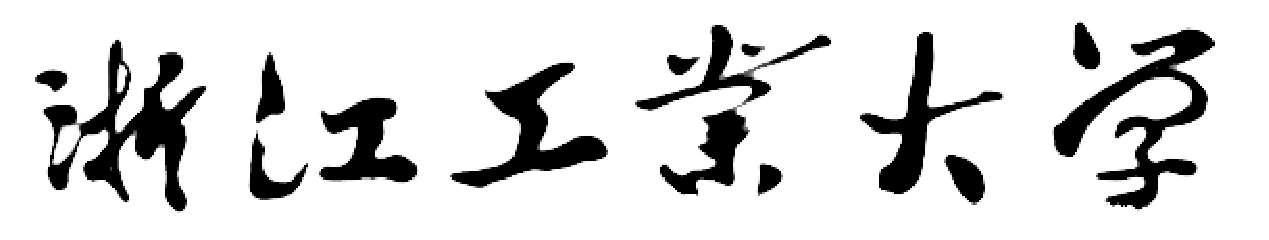
\includegraphics[width=98.40mm]{figures/zjut}
\end{center}
\vspace*{12mm}
\centerline{\songti\yihao{本科毕业设计说明书(论文)}}
\vspace*{8mm}
\centerline{\songti\xiaoer\textbf{(\zjutgrade\ 届)}}
\vspace*{7mm}
% 校徽
\begin{center}
  
\includegraphics[width=27.3mm]{figures/zjutlogo}
\end{center}

\vspace*{0.0mm}
\renewcommand{\arraystretch}{1.0}
\hspace*{12mm} 
{\songti\erhao{论文题目}}
\hspace{6mm} 
\begin{minipage}[t]{85mm} % 这里建议自行微调
    \linespread{1.1}{\songti\xiaoer\CJKunderline*{\zjuttitlec}}
\end{minipage}
\vspace*{1mm}
\begin{center}
    \setlength{\arrayrulewidth}{0.5pt}
    {\songti\sihao
        \renewcommand{\arraystretch}{1}
        \begin{tabular}{lc}
            作者姓名\qquad &  \zjutauthornamec \\ \cline{2-2}
            指导教师\qquad &  \zjutmentorc\\ \cline{2-2}
            \\
            学科(专业)\qquad &  \zjutmajor \\ \cline{2-2}
            所在学院\qquad &  \zjutcollegec \\ \cline{2-2}
            提交日期\qquad & \zjutsubmitteddatee \\ \cline{2-2}
        \end{tabular}
    }
\end{center}

  % 封面

\mainmatter\defaultfont\sloppy\raggedbottom

\begingroup % 在组内的chapter不换行
\let\clearpage\relax % chapter之后不换页
%%%%%%%%%% 摘要 %%%%%%%%%%
\titleformat{\chapter}{\centering\hei\sanhao\bfseries}{\chaptername}{1em}{} % 标题居中,黑体三号
% !Mode:: "TeX:UTF-8"

\chapter*{浙江工业大学本科生毕业设计外文翻译模板}
\noindent{\hei 摘要:}摘要是论文内容的高度概括,应具有独立性和自含性,即不阅读论文的全文,就能获得必要的信息。
摘要应包括本论文的目的、主要研究内容、研究方法、创造性成果及其理论与实际意义。
摘要中不宜使用公式、化学结构式、图表和非公知公用的符号和术语,不标注引用文献编号。避免将摘要写成目录式的内容介绍。\\
{\hei 关键词:}\quad 关键词~1;关键词~2;关键词~3;……;关键词~6(关键词总共~3~—~6~个,最后一个关键词后面没有标点符号)
%关键词~1;关键词~2;关键词~3;……;关键词~6(关键词总共~3~—~6~个,最后一个关键词后面没有标点符号)

\newline
\titleformat{\chapter}{\hei\sihao\bfseries}{\chaptername}{1em}{} % 恢复标题居左,黑体四号

%%%%%%%%%% 正文 %%%%%%%%%%
% !Mode:: "TeX:UTF-8"
\chapter{简介}

\section{为什么}

“为什么用\LaTeX{}{}?”

当把\LaTeX{}{}介绍给一个人的时候,这是面对的第一个问题。
当回答“它很好用时”,又会得到第二个问题:
“Word不好用吗?”答案当然是肯定的,
Microsoft Word\index{Word}是这个世界上目前最流行的,最易用的文字处理软件之一。

但是,
我这里要做一个转折了,如果是做过比较大的文档的,几十页以上,有分章,
分节,或者还要有页眉页脚页码目录以及封面这些东西,好吧,大部分人做过唯一的这种文档,那就是毕业论文了。
给毕业论文排版,几乎是大部分人的一场梦魇。如果性格里再带一点点追求完美的
念头,追求一点点排版的质量,那给自己的毕业论文排版,那一定会留下一生深刻的印象!

页码格式不对,页码编号不对,不同章节标题字体不一致,小标号缩进老对不齐,
数字有时候是Times Roman字体,
有的时候又成了宋体,有的段落前有一块空白,有的段落间距又太小。增加了一张图,
它后面图的标号又得重新来编一次,还有图的引用处也不要忘记……增加了一段文字,发现排好
的图又跑到下面一页去了。。。。。这一页留下了好大一片空白。下一页的表格又被它推
成了分布在两页。参考文献引用增加或者删除了一个,那就得找出全文要改动的所有引用处!!
什么,你是高级用户,会使用交叉引用,好吧,那有时候打出来的文档突然出现“错误!找不到引用--”
这样的字样,你是什么心情?
生成目录字体不一样,有的标题起的名太长,把页码挤到下一行去了,一个个改好了,一全更新又完了。
如果你的文档里还有一些公式,那又是一场战争了,有的公式字显得比正文大,有的又显得比正文小,
或者总是跟写的编号对不齐,不是偏上就是偏下。公式编辑器\index{公式编辑器}版本众多,换台电脑就只能看不能改了,
公式编辑器还经常提示已过期。blablabla……

千辛万苦,终于搞定了,看起来还算漂亮,到打印店去了,omg,word版本不对,版白排了,又乱了。
用PDF吧,不同软件生成的PDF总是跟原来的样子有点差距。做完论文,感觉是扒了一层皮。

\LaTeX{}解决了这个问题,它实际可以看成是一种写给机器的语言,把格式定义好,再填上内容,
它就会按设定好的格式把一份文档生成出来,一般是生成pdf文档,整个文档的格式首先是统一的,
不会出现不同章节的显示不一样的问题,并且,文档的格式可以是封装好的,使用的时候不需要
理会具体格式,直接可以使用,封闭格式这个功能留给会的人去做,写论文不需要关心太多的格式问题。

如果是往国外投文章,那么\LaTeX{}的应用更广泛,不少国外出版社直接提供其格式文件,
只要将文档头上的$\backslash$documentclass\{article\} 大括号里的“article”换成其相应的格式文件即可,
避开了格式调整问题。

话说回来,Word还是有优势的,所见即所得,上手容易,会鼠标键盘就会用。\LaTeX{}还是需要一些入门时间的,
如果单纯会使用这个模版,我想大约需要3个小时左右,如果会处理一些常见的程序错误以及做小的格式修改,
时间就会比较长了,大约要几天,有人引导的话会快一些。
Word在做小文档,比如就几页的文档上的优势\LaTeX{}{}是无法与之比拟的,做起来是很快,比如通知啦,传单啦。
但Word存在的意义应该不是就为了那几张小广告的,几百M的体积,几百RMB的价格,当然盗版很多。在这种应用
上还不如去用一下免费的WPS,或者OpenOffice。Word支持很多特性,支持宏,支持Visual Basic……,但是,它们
又太难了,不是随便一个人就会去有兴趣学它们的,学了很少有机会用到,屠龙之技。

\LaTeX{}{}还有两个优势是Word所没有的:
\begin{enumerate}
\item{文件体积小}

使用\LaTeX{}{},所要编辑的文件以“tex”为扩展名,如果用到参考文献,可能还需要扩展名为“bib”的参考文献数据库
文件,此外,还可能有的就是文档中要插入的图片文件了。
“tex”和“bib”文件都是纯文本文件,如果愿意,可以用记事本来编辑,按照一定的格式书写,格式也是很简单的,
看到了就会使用。
而Word文件是Microsoft自己定义的二进制文件,只有用Word软件或者其它兼容的软件打开,因为是Microsoft自己的二进制格式,
因此,体积会比较大,当然文件集成度很好,只有一个文件。
相比较之下\LaTeX{}{}可能有很多文件,但这个缺陷完全可以通过压缩软件打包来完成。
如果打开一个比较大的文档,机器破的话会比较慢,而且容易出一些错误导致Word意外关闭,想来各位都遇到过这种情况的吧。
文件如果发生了意外关闭,那就有可能被损坏,损坏后就有可能。。。。。打不开了,如果没有做一些备份,
那就成了“杯具”甚至“餐具”了。相较而言,\LaTeX{}{}的文件小,而且是纯文本文件,即使被损坏,
修复起来也比Word要容易得多。

\item{使写作更加专注于内容}

说实话,这一条在学会使用\LaTeX{}{}之前,我觉得是扯淡,那时的我觉得,使用Word边写边想也一样很快的。但在我学习使用\LaTeX{}{}
的过程中,我逐渐感受到,当只面对文本,不去想它下一段怎么排,什么样的格式时,思维更加连续,写起来也更快,
而且明显感觉到自己进入了一种写作的状态,这种感觉只在以前纸上写作感觉得到,专注于自己想的内容。
这一点,只有在学会使用之后,才能去体会得到。

\end{enumerate}


\section{模板说明}

ZJUTThesis~是为了帮助浙江工业大学本科毕业生撰写毕业论文而编写的~\XeLaTeX~论文模板,其前提是用户已经能处理一般的~\XeLaTeX~文档,并对~BibTeX~有一定了解,如果你从来没有接触过~\XeLaTeX~,建议先学习相关基础知识,磨刀不误砍柴工,能有助你更好使用模板\cite{huwei}。

由于作者水平有限,虽然现在的这个版本基本上满足了学校的要求,但难免存在不足之处,欢迎大家积极反馈,更希望浙江工业大学~\XeLaTeX~爱好者能一同完善此模板,让更多同学受益。

如有模板的疑问或有意向加入模板的维护和编写队伍中来,请给作者:Monster(diufanshu@gmail.com),或09级版本作者 Unlucky(unlucky1990@gmail.com)或MCKelvin(ibmmc@live.com)写信。


理论上,并不一定要把每章放在不同的文件中。但是这种自顶向下,分章节写作、编译的方法有利于提高效率,大大减少~Debug~过程中的编译时间,同时减小风险。

\section{下载安装}
本分支主页:~\url{https://github.com/diufanshu/zjutthesis}。除此之外,不再维护任何镜像。


\section{参考文献生成方法}

\LaTeX~具有插入参考文献的能力。Google Scholar~网站上存在兼容~BibTeX~的参考文献信息,通过以下几个步骤,可以轻松完成参考文献的生成。
\begin{itemize}
  \item 在\href{http://scholar.google.com/}{谷歌学术搜索}中,
        点击\href{http://scholar.google.com/scholar_preferences?hl=en&as_sdt=0,5}{学术搜索设置}。
  \item 页面打开之后,在\textbf{文献管理软件}选项中选择\textbf{显示导入~BibTeX~的链接},单击保存设置,退出。
  \item 在谷歌学术搜索中检索到文献后,在文献条目区域单击导入~BibTeX~选项,页面中出现文献的引用信息。
  \item 将文献引用信息的内容复制之后,添加到~references~文件夹下的~reference.bib~中。
\end{itemize}

\section{编译注意事项}
由于模板使用~UTF-8~编码,所以源文件应该保存成~UTF-8~格式,否则可能出现中文字符无法识别的错误。
  本模板中每一个~.tex~文件的文件的开头已经加上一行:\\
  \verb|% !Mode:: "TeX:UTF-8"|\\
     这样可以确保~.tex~文件默认使用~UTF-8~的格式打开。读者如果删去此行,很有可能会导致中文字符显示乱码。
     在~WinEdt~编辑器中可以使用以下两种方式保存成~UTF-8~格式

\section{系统要求}
    CTEX 2.9, MiKTeX 2.9 或者 TeX Live 2013。当然,新版本也是可以用的,注意宏包的更新。默认使用推荐的~WinEdt 7.0~编辑器可以完成文件的编辑和编译工作,或者直接用记事本也行,我用的是ST3+latextool,但这是盗版,需要面壁。。。

\section{\TeX~简介}

以下内容是~milksea@bbs.ctex.org~撰写的关于~\TeX~的简单介绍,略有改动。
注意这不是一个入门教程,不讲~\TeX~系统的配置安装,也不讲具体的~\XeLaTeX~代码。
这里仅仅试图以一些只言片语来解释:
进入这个门槛之前新手应该知道的注意事项,以及遇到问题以后该去如何解决问题。

\subsection{什么是 \TeX/\XeLaTeX,我是否应该选择它~?}

\TeX~是最早由高德纳(Donald Knuth)教授创建的一门标记式宏语言,
用来排版科技文章,尤其擅长处理复杂的数学公式。\TeX~同时也是处理这一语言的排版软件。
\XeLaTeX~是 Leslie Lamport 在~\TeX~基础上按内容/格式分离和模块化等思想建立的一集~\TeX~上的格式。

\TeX~本身的领域是专业排版领域
但现在~TeX/LaTeX~也被广泛用于生成电子文档甚至幻灯片等,~\TeX~语言的数学部分
偶尔也在其他一些地方使用。但注意~\TeX~并不适用于文书处理(Microsoft Office 的领域,以前和现在都不是)。

选择使用~\TeX/\XeLaTeX~的理由包括:
\begin{itemize}
\item 免费软件;
\item 专业的排版效果;
\item 是事实上的专业数学排版标准;
\item 广泛的西文期刊接收甚或只接收 LaTeX 格式的投稿;
\item[] ……
\end{itemize}
不选择使用~\TeX/\XeLaTeX~的理由包括:
\begin{itemize}
\item 需要相当精力学习;
\item 图文混合排版能力不够强;
\item 仅在数学、物理、计算机等领域流行;
\item 中文期刊的支持较差;
\item[] ……
\end{itemize}

请尽量清醒看待网上经常见到的关于~\TeX~与其他软件的优劣比较和口水战。在选择使用或离开之前,请先考虑
\TeX~的应用领域,想想它是否适合你的需要。


\subsection{我该用什么编辑器~?}

编辑器功能有简有繁,特色不一,从简单的纯文本编辑器到繁复的 Emacs,因人而易。基本功能有语法高亮、方便编译预览就很好了,扩充功能和定制有无限的可能。初学者可以使用功能简单、使用方便的专用编辑器,如 ~TeXWorks、Kile、WinEdt~等,或者类似所见即所得功能的~LyX;熟悉的人可以使用定制性更强的~Notepad++、SciTE、Vim、Emacs ~等。这方面的介绍很多,一开始不妨多试几种,找到最适合自己的才是最好的。

另外提醒一句,编辑器只是工作的助手,不必把它看得太重。

\subsection{我应该看什么~\XeLaTeX~读物~?}

这不是一个容易回答的问题,因为有许多选择,也同样有许多不合适的选择。
这里只是选出一个比较好的答案。更多更详细的介绍可以在版面和网上寻找(注意时效)。

近两年~\TeX~的中文处理发展很快,目前没有哪本书在中文处理方面给出一个最新进展的合适综述,
因而下面的介绍也不主要考虑中文处理。

\begin{enumerate}

\item 我能阅读英文。
\begin{enumerate}
\item 迅速入门:ltxprimer.pdf (LaTeX Tutorials: A Primer, India TUG)
\item 系统学习:A Guide to LaTeX, 4th Edition, Addison-Wesley
               有机械工业出版社的影印版(《\LaTeX{}~实用教程》)
\item 深入学习:要读许多书和文档,TeXbook 是必读的
\item 细节学习:去读你使用的每一个宏包的说明文档
\item 专题学习:阅读讲数学公式、图形、表格、字体等的专题文档
\end{enumerate}

\item 我更愿意阅读中文。
\begin{enumerate}
\item 迅速入门:lnotes.pdf (LaTeX Notes, 1.20, Alpha Huang)
\item 系统学习:《\LaTeXe{}~科技排版指南》,邓建松(电子版)
      如果不好找,可以阅读《\LaTeXe~入门与提高》第二版,陈志杰等,或者 《\LaTeXe~完全学习手册》,胡伟
\item 深入学习:~TeXbook0.pdf~(特可爱原本,TeXbook 的中译,xianxian)
\item 具体问题释疑:~CTeX-FAQ.pdf~,\\
        吴凌云,~\url{http://www.ctex.org/CTeXFAQ}~
\end{enumerate}
\end{enumerate}

遇见问题和解决问题的过程可以快速提高自己的技能,建议此时:
\begin{itemize}
  \item 利用~Google~搜索。
  \item 清楚,扼要地提出你的问题。
\end{itemize}

\subsection{什么知识会过时~?什么不会~?}

\TeX~是排版语言,也是广泛使用的软件,并且不断在发展中;
因此,总有一些东西会很快过时。作为学习~\TeX~的人,
免不了要看各种各样的书籍、电子文档和网络论坛上的只言片语,
因此了解什么知识会迅速过时,什么知识不会是十分重要的。

最稳定的是关于~Primitive \TeX~和~Plain \TeX~的知识,也就是 Knuth
在他的《The TeXbook》中介绍的内容。因为~\TeX~
系统开发的初衷就是稳定性,要求今天的文档到很久以后仍可以得到完全相同的结果,
因此 Knuth 限定了他的~\TeX~语言和相关实现的命令、语法。这些内容许多年来就没有多少变化,
在未来的一些年里也不会有什么变化。
Primitive \TeX~和 Plain \TeX~的知识主要包括 \TeX~排版的基本算法和原理,
盒子的原理,底层的 \TeX~命令等。其中技巧性的东西大多在宏包设计中,
初学者一般不会接触到很多;而基本原理则是常常被提到的,
譬如,~\TeX~把一切排版内容作为盒子(box)处理。

相对稳定的是关于基本~\LaTeXe~
的知识,也包括围绕~\LaTeXe~的一些核心宏包的知识。
在可预见的将来,~\LaTeXe~不会过时。
\LaTeXe~的知识是目前大部分~\LaTeX~书籍的主体内容。关于~\XeLaTeX~的标准文档类
~(article、report、book、letter、slide~等),关于基本数学公式的输入,
文档的章节层次,表格和矩阵,图表浮动体,LR 盒子与段落盒子……
这些~\XeLaTeX~的核心内容都是最常用的,相对稳定的。
与~\LaTeXe~相匹配的核心宏包,
如~graphics(x)、ifthen、fontenc、doc~等,也同样是相对稳定的。
还有一些被非常广泛应用的宏包,如~amsmath~系列,也可以看作是相对稳定的。

简单地说,关于基本~\TeX/\XeLaTeX~的语言,都是比较稳定的。与之对应,实现或者支持~\TeX/\XeLaTeX~语言的软件,
包括在~\TeX/\XeLaTeX~基础上建立的新的宏,都不大稳定。

容易过时的是关于第三方~\XeLaTeX~宏包的知识、第三方~\TeX~工具的知识,以及新兴~\TeX~相关软件的知识等。
~\TeX~和~\XeLaTeX~语言是追求稳定的;但无论是宏包还是工具,作为不断更新软件,它们是不稳定的。
容易过时的技术很多,而且现在广泛地出现在几乎所有~\XeLaTeX~文档之中,因此需要特别引起注意:
宏包的过时的原因可能是宏包本身的升级换代带来了新功能或不兼容,
也可能是同一功能的更新更好的宏包代替了旧的宏包。前者的典型例子比如绘图宏包~PGF/TikZ~,
现在的~2.00~版功能十分强大,和旧的~1.1x~版相差很大,和更旧的~0.x~版本则几乎完全不同;后
者的典型例子比如~caption~宏包先是被更新的~caption2~宏包代替,后来~caption~宏包更新又使得
caption2 宏包完全过时。——安装更新的发行版可以避免使用过旧的宏包;
认真阅读宏包自带的文档而不是搜索得到的陈旧片断可以避免采用过时的代码。

工具过时的主要原因也是升级换代和被其他工具替换。前者的典型例子是编辑器
WinEdt~在~5.5~以后的版本支持~UTF-8~编码,而旧版本不支持;
后者的典型例子是中文字体安装工具从~GBKFonts~到~xGBKFonts~到~FontsGen~不断被取代。
图形插入是一个在~\TeX~实现、宏包与外围工具方面都更新很快的东西。
在过去,最常用的输出格式是~PS(PostScript)~格式,因此插入的图像以~EPS~为主流。
使用~Dvips~为主要输出工具,外围工具有~GhostScript、bmeps~等等,相关宏包有~graphics~等,
相关文档如《\LaTeXe{}~ 插图指南》。

\XeLaTeX~不限定图片格式,推荐使用EPS格式的图片,但是PNG和JPEG格式的图片也支持。

值得特别提出注意的就是,中文处理也一起是更新迅速、容易过时的部分。
而且因为中文处理一直没有一个“官方”的“标准”做法,软件、工具、
文档以及网上纷繁的笔记也就显得相当混乱。从八十年代开始的~CCT~系统、
天元系统,到后来的~CJK~方式,到近来的~XeTeX~和~LuaTeX~ 方式,
中文处理的原理、软件、宏包、配置方式等都在不断变化中。

\section{免责声明}

本模板依据《浙江工业大学本科生毕业设计说明书(论文)模板》编写,作者希望能给使用者写作论文带来方便。然而,作者不保证本模板完全符合学校要求,也不对由此带来的风险和损失承担任何责任。
% !Mode:: "TeX:UTF-8"

\chapter{开发框架的主要技术}
\section{代码和配置的层与层之间的分离}
Web应用程序有各种设计问题,如表现,商业逻辑,数据存取和安全性。不同的代码层的分离设计有如下几个方面的优势,如:便于维修,实施良好设计模式的能力,选择专门的工具的能力和具体问题的解决技术。将一个项目进行层与层之间的分离导致了这些层之间的依赖关系。例如,一个简单的使用案例,它涉及数据的输入和查询通常必须整合表示,业务逻辑和数据访问以达到所需的功能[3] 。因此,必须有一个明确的策略来管理这些依赖关系。开发框架包括设计模式,可复用的代码和配置文件,使开发框架尽可能地容易的被使用。这一框架使用Spring的反向控制来管理相依。 Spring框架[4]提供了一种方法整合各层成为一个应用项目。它通过Spring应用上下文来完成这一目标,这是一个对象之间管理依赖策略。Spring使用的依赖注入和拦截技术介绍如下。

我们所写的代码依赖于使用的对象。它负责创建这些对象。这可能导致紧耦合的,但我们希望我们的代码是松散耦合。依赖注入是一个技术,可以帮助我们实现这一目标。依赖注入是反向控制(IOC)的一种形式[5]。当应用程序使用依赖注入时,代码将变得更加清洁和容易。这就是松耦合,从而更容易配置和测试。开发框架使用了多个Spring应用背景文件来定义层与层之间的依赖关系。方法拦截是面向方面编程(AOP)概念[6]。Spring AOP方法拦截是通过JDK动态代理来实现的。开发框架使用Spring AOP来管理问如交易管理和性能监测等问题。

开发框架包括两个不同的部分:代码和配置。代码位于一个特定的应用层,并侧重于某一特定条件中的应用解决方案。这可能要与数据库交互,或将数据显示给屏幕。配置将应用的各个层联系在一起。从代码中分离出配置使我们能够独立管理配置,使我们在同一代码基础上方便的进行不同的配置。例如,数据访问对象(DAO)知道它是使用JDBC通过数据源来连接一个数据库的,但它不知道该数据源是如何实现的。它可能是一个Java命名和目录接口(JNDI上下文或是来自驱动程序。它可以指向远程数据库或本地数据库。无论数据来自何处,DAO执行操作数据源的方式是相同的。同样,服务对象可能依赖于DAO ,但不知道DAO是如何实现,可能通过Hibernate,直接的JDBC ,或Web服务。互动服务对象与DAO有相同的方式,而不管DAO的实现。

Spring通过Spring应该上下文来管理我们的应用程序的整个配置,这些配置是一些XML文件。我们可以在一个文件中定义应用的环境。然而,我们可以在较小的文件中定义它来简化配置管理。这样的应用环境文件的逻辑集合组成了一个被称之为配置集的完整的应用配置。

开发基于Java的企业应用的标准配置是在一个框架的配置中设置使用如数据源和JNDI的资源的外部资源。这种类型的配置有些时候可能带来如下问题:(1)尚未加载完全的数据库。开发人员可能要测试某些类型的数据的显示,但如果基础数据尚未完成,他们将无法做到这一点。(2)服务或DAOs可能还未被开发。整合未完成的服务或DAOs可能阻碍发展的进程。

这些问题降低了生产力。开发框架已从它的代码中分散其配置,我们可以针对开发使用有选择的配置集。这可以减轻我们对外部系统的可用性的担心,这对于解决开发的中间需求是不相关的。

开发框架定义了两种配置集:默认和独立。我们还可以自定义应用,来增加基于我们项目需要的额外配置集。默认配置使用在JNDI中的定义的数据源来连接数据库。它完全使用了应用服务和DAOs 。独立的配置设置对开发而言是最灵活的。此配置集:(1)使用DriverManagerDataSource连接到任何本地安装的数据库或开发数据库;(2)使用Spring的DataSourceTransactionManager作为本地事务管理;(3)利用充分开发应用服务和DAOs;(4)充分利用Spring应用上下文在应用服务器以外进行运行和测试。

开发框架通过它的应用上下文进行配置。应用上下文被定义一个或多个XML文件。一个配置集是定义一个应用上下文的一套XML文件。配置集包括两部分:服务和网络。该服务定义了整合过程中的DAOs和资源。一个配置不能同时完成这些部分。

开发框架配置集通过被Spring称之为bean映射上下文组合到一起,这些映射在beanRefContext.xml和applicationContextMapping.properties 中定义。beanRefContext.xml文件定义所有的配置的服务部分。此文件位于的src /服务项目的配置目录下。应用上下文之间共享也是通过这个目录下的配置来实现的。此外,各配置有自己的子目录,其中包含自己的特定配置。例如服务和DAOs 通过配置集来共享,而支持服务(如数据源)则属于子目录。 XML文件在应用程序通过使用<bean>标记来定义Spring bean。Spring bean是一个Java对象和通过应用上下文来初始化。

\section{类及其关系}
利用开发框架,在一个典型项目中有如下的代码和配置:(a)Action,ActionForm类和validation.xml文件;(b)服务接口和实现类;(c)DAO接口和实现类;(d)以上这些的关系管理。当我们开始我们例子的开发时,我们必须认识到所有这些类和他们的关系的重要性。

\section{测试技术}
测试应是项目开发过程中的一个不可分割的组成部分的。使用开发框架建立的应用程序,单元测试是指只测试服务或集成层的单一类。表现层(Action类)不执行单元测试。这种测试的目的是保证每个类的行为封装与预期一致。项目中的单元测试是基于JUnit框架的[7]。与单元测试不同,集成测试需要测试代码之间的相互依赖性。这种测试的目的是以确保各个不同的类(不同的开发者开发的)整合在一起时也能想期望一样的运作。在功能测试过程中,重点是采用不同的场景进行功能的测试。典型的功能测试包括在业务层用不同的数据进行类的测试。

为了执行不同类型的测试,项目在开发过程中必须是测试可测试的。下面列出的可测试项目的一些基本特性。(1)开发单元的简单和集成测试。我们可以在没有数据源,或排队的情况下执行单元测试。当然,我们也能模拟相依赖代码而进行测试。(2)有易于进程各种模拟测试场景的功能测试。(3)在整个生命周期中方便重新运行所有测试。(4)从应用代码中清楚的分离出测试代码来。

精心计划应用的各个设计问题,如表示,服务和数据访问对于可测试的应用是非常重要的。应用程序编码以get方法、set方法、变量等开始。单元测试是是其他任何测试方法的基础。开发框架设计的便利的可测试应用开发的方法:提供测试模板类来帮助建立单元测试,使应用更易于配置以适应测试需求。单元测试可以运行像任何JUnit测试。默认的专门开发的“建设脚本”提供了一个任务来运行单元测试。这个任务部署的EAR文件,可以单独运行。

\section{页面表示设计}
开发框架采用Struts框架和JavaScript来实现页面,并提供可扩展用于另外项目的额外功能。当使用Struts框架进行发展,首先,我们在web.xml配置Servlet Action;然后在struts-config.xml中配置action mapping,form bean 和local forwards;最后我们在validation.xml配置验证规则。
这种建立应用程序的方法在开发框架中已经发生了改变,开发人员不必要直接编辑config.xml或validation.xml文件。相反,我们通过XDoclet注释直接在Action和Action Form类中直接配置。这些信息在运行Ant脚本时翻译插入struts-config.xml和validation.xml文件中。
有两种需要验证的类型:数据格式验证和业务逻辑验证。数据格式验证最好在表示层进行,而业务逻辑验证最好的在服务层进行验证。在业务层发生的业务逻辑错误,必须通过抛出异常进行处理。
以下是表现层的设计目标:(1)每个JSP文件只有一个Action类和ActionForm类。一个单一动作类必须处理一个单一的页面;(2)使用XDoclet定义依赖和验证规则;(3)开发人员应该避免或尽量减少使用sessoin对象,因为它阻碍了可扩展性。
开发框架提供了一个默认的Action模板类,其中包含解决上述设计目标的方法。以下是典型的开发web页面所需要的代码:(1)创建一个带有称之为“actionType”默认隐藏域的JSP文件,用于处理在页面上发生的用户行为。(2)创建一个扩展模板Action类的新的Action类。我们必须使用XDoclet配置ActionForm和服务类之间的关联。然后,我们就应该针对隐藏域“action Type”中的值来建立具体的处理用户动作方法。最后,我们根据需要给这个Actoin类访问权限。这就是Spring的配置文件所做的工作。(3)创建一个新的ActionForm类,并用XDoclet注释指定验证规则。
一旦JSP,Action和ActionForm创建完成,就必须运行Ant脚本来重新生成“struts-config.xml”文件。
\section{数据库访问}
通过框架建立的应用程序支持直接使用JDBC和Hibernate框架将数据持久化到关系数据库中。应用程序通过Spring上下文文件进行配置。直接使用JDBC的DAOs必须继承Spring框架中的JdbcDaoSupport.java类。同样,使用Hibernate的DAOs必须继承Spring框架的HibernateDaoSupport.java类。

\section{通过注释进行配置}
开发框架使用Spring框架维持代码之间依赖。一些相依(例如Action和ActionForm )在“struts-config.xml”中配置,而另一些(例如服务和DAO)在Spring应用上下文文件(applicationContext.xml)中配置。在一个团队中这些配置文件可以被开发者共享。就这是为什么在这些配置上可能发生版本冲突。开发框架提供了一种新的有效的办法,使用特别注释来定义这些依赖。通过使用这些注释,配置变得更加简单和相互冲突也可以避免。

% !Mode:: "TeX:UTF-8"

\chapter{开发框架中的服务}
开发框架提倡使用plain-old-java-object(POJOs)实现业务逻辑。业务逻辑必需申明为接口。所有服务的实现必须实现一个或多个业务接口当有业务规则验证错误服务层抛出业务异常这是推荐的。开发框架采用基于Spring框架的事务处理方法[8]。这是通过面向方面编程(AOP)实现的。

开发框架提供了从服务接口(与应用程序的业务逻辑联系)分离部署接口(与服务消费者联系)的良好实践。在WDSL中部署接口是Java接口表示服务的外在表现。实现这个接口的类必须代表实现服务实现接口的类的需要。这样可确保所有的业务逻辑是保持在一个正确的地方。服务接口是一种Java接口,代表宝物逻辑。在大多数情况下,部署接口包含从服务接口而来的一个方法子集。

Apache Axis 1.2.4 Web服务框架是目前Web服务的标准。开发Web服务,有两种不同的方法[9]:contract first和contract last。Contract first与contract last的区别WDSL首先被创建还是从代码中生成。
当服务消费者或供应商的外部供应商时,他们可以使用不同的技术实现WEB服务(他们可以使用.NET不是Java)[10]时,Contract first办法对开发WEB服务是一个很好的做法。

% !Mode:: "TeX:UTF-8"

\chapter{中间层的集成}
与外部资源的整合有多种技术,如数据库和Web服务。开发框架使用在逻辑层称之为“整合”层的技术。这一层的设计目标是:(1)通过JDBC或Hibernate进行的数据库访问必须封装在数据存取对象(DAO)中。(2)Web服务应尽可能简单。(3)所有的外部数据格式转换到应用程序域对象应限于这一层。(4)在这个层单元测试类应用做的简单。

开发框架支持使用Hibernate和直接的JDBC调用访问关系数据库。使用Spring框架的模板类:JdbcTemplate和HibernateTemplate是推荐的。当直接使用JDBC访问关系型数据库,建议应用程序的DAOs继承自Spring框架的JdbcDaoSupportJdbcTemplate类管理访问数据库(例如PreparedStatement)的资源。开发框架使用应用程序配置文件将datasource插入到DAOs。当使用Hibernate访问关系数据库,通过应用程序配置文件将Hiberate SessionFactory注入到应用程序的DAOs。

% !Mode:: "TeX:UTF-8"

\chapter{开发生命周期}
开发框架的重点在一个开发团队中可以明确定义角色及其相互作用的结构上。三种角色描述如下。这些角色的相互作用是整个应用项目成功的关键。(a)前端的开发人员专注于JSPs,Action/ActionForm类和外部Web服务。(b)服务的开发者专注于开发应用的服务和整合这些服务中的不同部分。(c)项目集成者主要专注开发的集成文件,如DAOs或消费型Web服务。

发展中的一个基本问题是在其依赖组件没有准备好或不可用时如何开发和集成的代码。开发框架通过以声明式注入“模拟对象”这种结构来解决这个问题,并在开发生命周期的过程中用实际对象取代模拟对象。由于我们的应用是通过不同的配置集进行配置的使这成为了可能。该框架使团队能测试开发过程中的一个组成部分。这使编写和运行JUnit测试成为了可能。框架专注于测试应用服务和他们的依赖性。应用部署在一个单一的Enterprise Archive(EAR)文件中。Ant脚本生成此EAR文件,并可以手动运行或定期调度。建议在创建EAR之前运行所有的JUnit测试。

% !Mode:: "TeX:UTF-8"

\chapter{总结}
本文作者概述了J2EE开发框架。作者讨论了J2EE项目中重要的架构问题,技术和发展步骤。这些资料来自实际的项目经验,是为了帮助开发人员构建基于J2EE系统和设计自己的框架。然而,这仅仅是冰山的一角,短短的文章不足以详细描述J2EE在科学和企业应用,特别是基于Web的非线性分析仿真软件的潜在影响。


\endgroup % 组结束
%%%%%%%%%% 参考文献 %%%%%%%%%%
\clearpage % 显式换页,使书签定位准确
\defaultfont
\bibliographystyle{GBT7714-2005NLang-ZJUT}
\phantomsection
\markboth{参考文献}{参考文献}
\addcontentsline{toc}{chapter}{参考文献}       % 参考文献加入到中文目录
\nocite{*}                                     % 若将此命令屏蔽掉,则未引用的文献不会出现在文后的参考文献中。
\bibliography{references/reference}

\end{document}
